\documentclass[12pt,a4paper]{article}
\usepackage[margin=1in]{geometry} % 设置页面边距
\usepackage{graphicx} % 插入图片
\usepackage{amsmath} % 数学公式
\usepackage{listings} % 代码块
\usepackage{caption} % 图表标题
\usepackage{booktabs} % 表格线条
\usepackage{ctex} % 中文支持
\usepackage{subcaption} % 多个子图或表格
\usepackage{array} % 数组和表格
\usepackage{multirow} % 多行合并的表格
\usepackage{parskip}
\usepackage{float}
\setlength{\parindent}{0pt}

\geometry{a4paper, margin=2.5cm} % 设置页面边距

\title{实验报告:人工智能导论-分类实践}
\author{张立博 2021012487}
\date{\today}

\begin{document}
\maketitle

\section{引言}
在本实验中,我们研究了分类实践,并尝试了不同的模型和超参数配置。本报告旨在评估模型的性能和计算效率,并展示实验结果。

\section{方法}
\subsection{数据集}
本次作业使用的数据集是推特的情感分析数据集。

\subsection{模型选择}
在本次实验中,我选择了几种常用的机器学习模型,分别为决策树、逻辑回归、随机森林和KNN,并根据实验要求对模型进行了调参。前三种模型为sklearn库官方实现,KNN模型为基于助教提供的框架手动实现。

\subsection{超参数调优}
为了获得最佳性能,我使用了网格搜索和K折交叉验证来选择模型的最佳超参数配置。

\subsection{其他机器学习技术}
在助教提供的库之外,我使用了$scikit-learn$ 库中的$sklearn.model\_selection.GridSearchCV$类辅助进行网格搜索和交叉验证。它提供了一个方便的接口,用于系统地搜索给定模型的超参数空间,并使用交叉验证评估每个超参数组合的性能。

\section{实验结果}
\subsection{模型性能评估}
基于网格搜索和交叉验证的超参数调优过程计算成本较高,由于算力和时间有限
所以对于每个模型本实验只对有限维度和有限范围的超参数进行了组合,
在训练集上训练模型,并在验证集上评估性能,最终选择最佳的超参数配置。
\subsubsection{决策树}
对于决策树模型,我对以下超参数进行了调整:\\
$- \texttt{max\_depth}$:决策树的最大深度,选择了3个取值:2、3、4、None。\\
$- \texttt{criterion}$:划分标准,选择了2个取值:gini、entropy。\\
在不同参数组合下,决策树模型的准确度如表1所示:\\
\begin{table}[H]
    \centering
    \caption{决策树模型准确度}
    \label{tab:dt_performance}
    \begin{tabular}{ccc}
      \toprule
      max\_depth & criterion & 准确度 (\%) \\
      \midrule
      2 & gini &  29.12 \\
      3 & gini &  28.78 \\
      4 & gini &  29.00 \\
      None & gini &  31.25 \\
      2 & entropy &  29.12 \\
      3 & entropy &  28.45 \\
      4 & entropy &  29.16 \\
      None & entropy &  31.40 \\
      \bottomrule
    \end{tabular}
  \end{table}
对应的参数组合-准确度图示如下:
\begin{figure}[H]
    \centering
    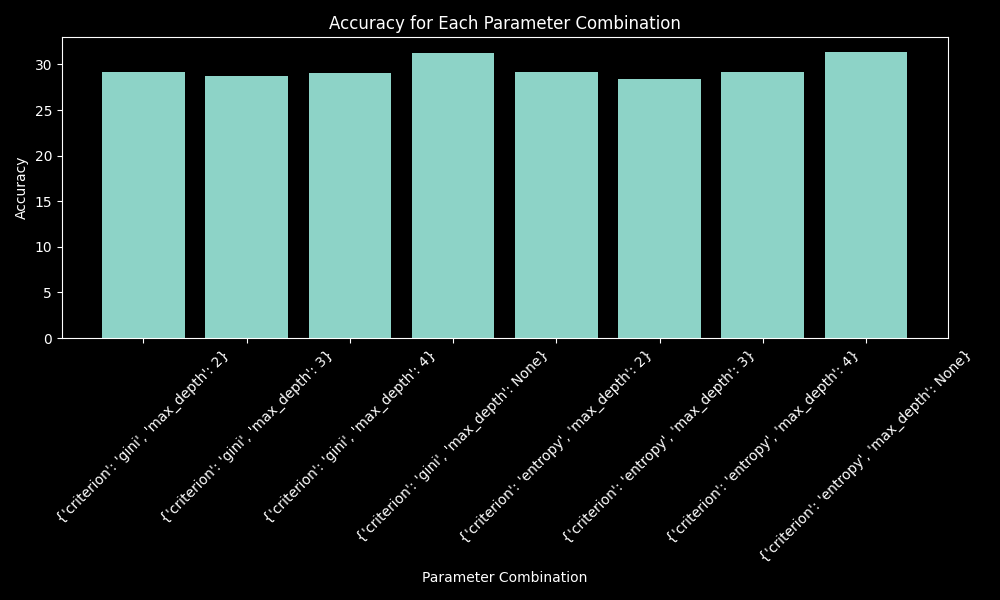
\includegraphics[width=0.65\textwidth]{plot1.png}
    \caption{不同参数组合下的准确率}
    \label{fig:accuracy}
  \end{figure}
从表中可以看出,参数组合为$criterion = entropy, max\_depth=None$时决策树模型的准确度有最好的表现,达到了 31.4\%。

\subsubsection{随机森林}
对于随机森林模型,我对以下超参数进行了调整:\\
$- \texttt{max\_depth}$:决策树的最大深度,选择了3个取值:5、10、None。\\
$- \texttt{n\_estimators}$:决策树的数量,选择了3个取值:100、200、300。\\
通过对这些超参数进行组合,得到了如下表格中所示的结果。\\
在不同参数组合下,随机森林模型的准确度如表2所示:

\begin{table}[H]
    \centering
    \caption{随机森林模型准确度}
    \label{tab:rf_performance}
    \begin{tabular}{ccc}
      \toprule
      n\_estimators & max\_depth & 准确度 (\%) \\
      \midrule
      100 & 5 & 33.59 \\
      100 & 10 & 34.84 \\   
      100 & None & 36.50 \\
      200 & 5 & 33.21 \\
      200 & 10 & 34.51 \\
      200 & None & 36.56 \\
      300 & 5 & 33.24\\
      300 & 10 & 34.59 \\
      300 & None & 36.66 \\
      \bottomrule
    \end{tabular}
  \end{table}
  对应的参数组合-准确度图示如下:
\begin{figure}[H]
    \centering
    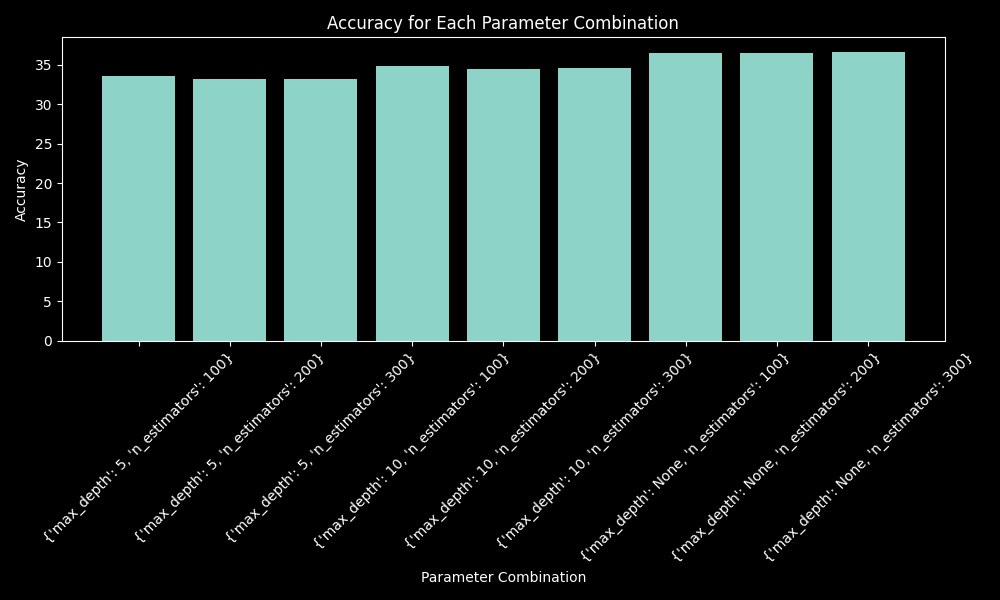
\includegraphics[width=0.65\textwidth]{plot3.png}
    \caption{不同参数组合下的准确率}
\end{figure}
从表中可以看出,参数组合为$n\_estimators=300, max\_depth=None$时随机森林模型的准确度有最好的表现,达到了36.66\%。

\subsubsection{逻辑回归}
对于逻辑回归模型,我对以下超参数进行了调整:\\
$- \texttt{penalty}$:正则化项的类型,选择了两种取值:l1和l2。\\
$- \texttt{C}$:正则化强度的倒数,选择了6个取值:0.001、0.01、0.1、1、10、100。\\
$- \texttt{solver}$:优化算法,选择了两种取值:liblinear和saga。\\
在不同参数组合下,逻辑回归模型的准确度如表3所示:

\begin{table}[H]
    \centering
    \caption{逻辑回归模型准确度}
    \label{tab:lr_performance}
    \begin{tabular}{cccc}
    \toprule
    penalty & C & solver & 准确度 (\%) \\
    \midrule
    l1 & 0.001 & liblinear & 33.17 \\
    l1 & 0.001 & saga & 33.73 \\
    l1 & 0.01 & liblinear & 34.74 \\
    l1 & 0.01 & saga & 34.81 \\
    l1 & 0.1 & liblinear & 34.65 \\
    l1 & 0.1 & saga & 34.56 \\
    l1 & 1 & liblinear & 34.63 \\
    l1 & 1 & saga & 34.55 \\
    l1 & 10 & liblinear & 34.62 \\
    l1 & 10 & saga & 34.56 \\
    l1 & 100 & liblinear & 34.62 \\
    l1 & 100 & saga & 34.56 \\
    l2 & 0.001 & liblinear & 34.87 \\
    l2 & 0.001 & saga & 34.67 \\
    l2 & 0.01 & liblinear & 34.67 \\
    l2 & 0.01 & saga & 34.57 \\
    l2 & 0.1 & liblinear & 34.62 \\
    l2 & 0.1 & saga & 34.56 \\
    l2 & 1 & liblinear & 34.62 \\
    l2 & 1 & saga & 34.55 \\
    l2 & 10 & liblinear & 34.63 \\
    l2 & 10 & saga & 34.55 \\
    l2 & 100 & liblinear & 34.63 \\
    l2 & 100 & saga & 34.55 \\
    \bottomrule
    \end{tabular}
    \end{table}
对应的参数组合-准确度图示如下:
\begin{figure}[H]
    \centering
    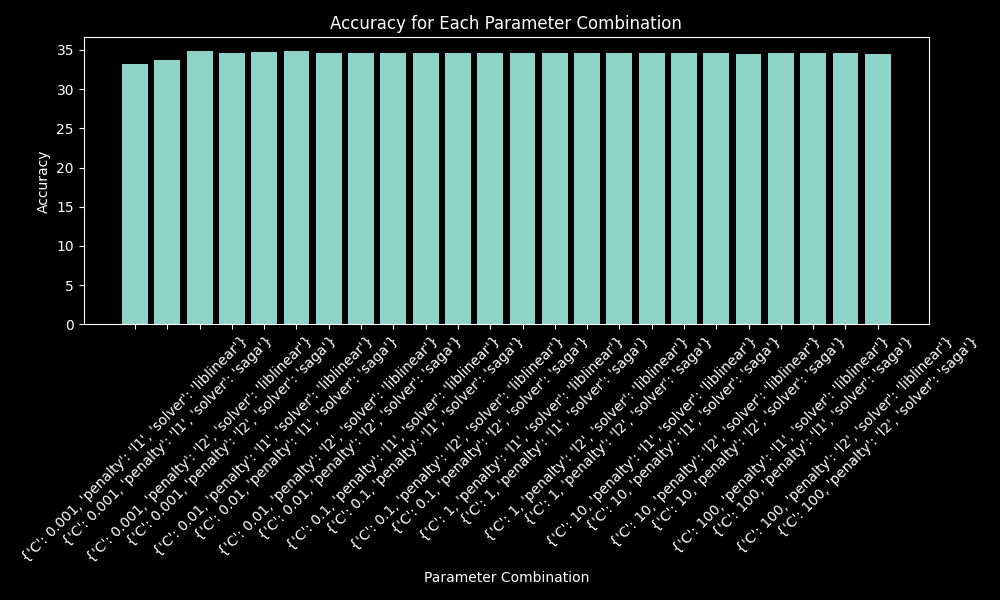
\includegraphics[width=0.65\textwidth]{plot2.png}
    \caption{不同参数组合下的准确率}
\end{figure}
从表中可以看出,参数组合为$C=0.001, penalty = l2, solver = liblinear$时逻辑回归模型的准确度有最好的表现,达到了34.87\%。

\subsubsection{K近邻}
对于K近邻模型,我对以下超参数进行了调整:\\
$- \texttt{n\_neighbors}$:最近邻居的数量,选择了3个取值:3、5、7。\\
$- \texttt{metric}$:距离度量方式,选择了3种取值:欧氏距离(euclidean)、曼哈顿距离(manhattan)、闵可夫斯基距离(minkowski)。\\
在不同参数组合下,K近邻模型的准确度如表4所示:

\begin{table}[H]
    \centering
    \caption{K近邻模型准确度}
    \label{tab:knn_performance}
    \begin{tabular}{ccc}
      \toprule
      n\_neighbors & metric & 准确度 (\%) \\
      \midrule
      3 & euclidean & 76.21 \\
      3 & manhattan & 79.18 \\
      3 & minkowski & 76.21 \\
      5 & euclidean & 72.61 \\
      5 & manhattan & 76.53 \\
      5 & minkowski & 72.61 \\
      7 & euclidean & 68.92 \\
      7 & manhattan & 72.58 \\
      7 & minkowski & 68.92 \\
      \bottomrule
    \end{tabular}
\end{table}
对应的参数组合-准确度图示如下:
\begin{figure}[H]
    \centering
    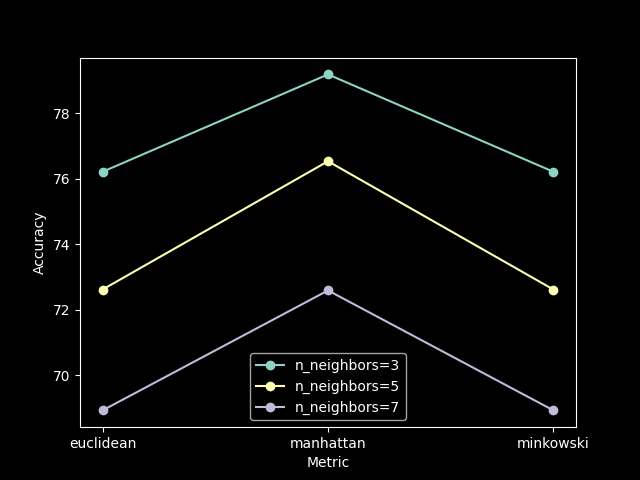
\includegraphics[width=0.65\textwidth]{plot4.png}
    \caption{不同参数组合下的准确率}
\end{figure}
从表中可以看出,参数组合为$n\_neighbors = 3, metric = manhattan$时K近邻模型的准确度有最好的表现,达到了79.18\%。

\subsection{计算效率评估}
在实验中对具有上述最佳参数组合的各模型进行训练与预测,对应的时间统计如下:
\begin{table}[H]
    \centering
    \caption{各模型计算效率评估}
    \label{tab:efficiency}
    \begin{tabular}{cc}
      \toprule
      模型 & 训练+预测时间 (秒)\\
      \midrule
      决策树 & 2.0941\\
      随机森林 & 60.3114\\
      逻辑回归 & 0.6485\\
      K近邻 & 439.2211\\
      \bottomrule
    \end{tabular}
\end{table}
对各模型计算效率进行理论分析
\subsubsection{决策树}
决策树的构建过程相对高效,它的计算复杂度主要取决于训练数据的数量和特征的数量。
决策树的训练时间复杂度为$O(nmlog(m))$,其中n是训练样本的数量,m是特征的数量。
在树的搜索过程中,预测的时间复杂度为$O(log(m))$,其中m是树的深度。
\subsubsection{随机森林}
随机森林是通过集成多个决策树来提高算法的准确性。
随机森林的训练时间复杂度取决于决策树的数量和树的深度。
相比于单个决策树,随机森林的训练时间要长一些,因为需要构建多个决策树。
预测时,需要遍历每个决策树来获得最终的预测结果。因此,预测时间复杂度与决策树数量成正比。
\subsubsection{逻辑回归}
逻辑回归是一种线性分类模型,它的计算效率通常很高。
逻辑回归的训练时间复杂度取决于训练样本的数量和特征的数量。
训练时,逻辑回归通过迭代算法来拟合参数,通常使用梯度下降法。
预测时,逻辑回归的计算复杂度很低,只需要进行一次矩阵乘法运算。
\subsubsection{K近邻}
K近邻算法的计算效率相对较低,特别是在处理大型数据集时。
训练阶段的计算复杂度很低,因为只需将训练样本存储起来。
预测时,需要计算每个测试样本与所有训练样本之间的距离,并找到最近的K个邻居。
这个过程需要较多的计算资源,尤其是在高维数据集中。\\
\\
可以看出,理论分析与实验结果比较相符,在本实验数据集下,计算效率由高到低依次为逻辑回归>决策树>随机森林>K近邻。\\
同时,不同的参数组合对模型的计算效率也有较大影响,但由于算力和时间有限,本次实验只统计了3.1中各最佳模型的训练和预测时间。
\subsection{最终结果}
最终在测试集上评估了各最佳模型的性能,各模型的准确度如下表:
\begin{table}[H]
    \centering
    \caption{模型在测试集上的准确度}
    \label{tab:accuracy}
    \begin{tabular}{ccc}
      \toprule
      模型 & 准确度 (\%) \\
      \midrule
      决策树 & 89.1 \\
      随机森林 & 92.0 \\
      逻辑回归 & 41.0 \\
      K近邻 & 90.2 \\
      \bottomrule
    \end{tabular}
  \end{table}
可以看出,决策树,随机森林和手动实现的K近邻模型在测试集上的准确度较高,而逻辑回归准确度较低。
可能是因为逻辑回归模型对特征依赖较强,对样本分布的假设较为严格,对于特征表示不够准确或信息丢失较多,非线性或类别不平衡的情感分类问题表现较差。
同时,各模型在测试集上的准确度明显大于在验证集上的准确度,可能是因为数据分布不一致,验证集规模较小等。
\section{结论}
在本次实验中,通过对分类问题进行实践,我探索了决策树、随机森林、逻辑回归和K近邻等不同模型的性能和效率。
深入理解了不同模型的性能和效率特点。探索了超参数调优、模型评估和计算效率分析等关键步骤,为后续的模型选择和应用提供了重要参考。
\end{document}
